\section{Experimental Evaluation}
\label{sec:experiments}

Experimental validation should demonstrate that online measurements of the real-time system match with the timing analysis results in a way that the timing analysis results are always close but conservative. One of the biggest assumptions in our CPN work is the knowledge of worst-case execution times of the individual steps in the component operations. We have previously designed \cite{SEUS} a business-logic modeling grammar that captures the temporal behavior of component operations, especially WCET metrics for the different code blocks inside an operation. For example, consider a simple \emph{remote method invocation} (RMI) application as shown in Figure \ref{fig:rmi_application}. The client component is periodically triggered by an internal timer and executes a synchronous remote method invocation to a remote server component. The interaction here demands that the client component be blocked for the duration of time it takes the server to receive the operation, process its message queue, execute the relevant callback, and respond with output. 

Note that in Figure \ref{fig:rmi_application}, we only annotate isolated code blocks that take a fixed amount of execution time on a specific hardware architecture. These are the only measurements that we can reliably make with repeated testing and instrumentation. The client-side blocking delay is not measured because the number of factors responsible for this delay are numerous e.g. server's message queue state, scheduling non-determinism, network delays etc. In order to be able to predict this delay, we need to use state space analysis and search through the tree of possible executions to identify the worst-case blocking delay. This also means that our CPN model must capture and account for such delay-causing factors.
 

\begin{figure}[ht]
	\centering
	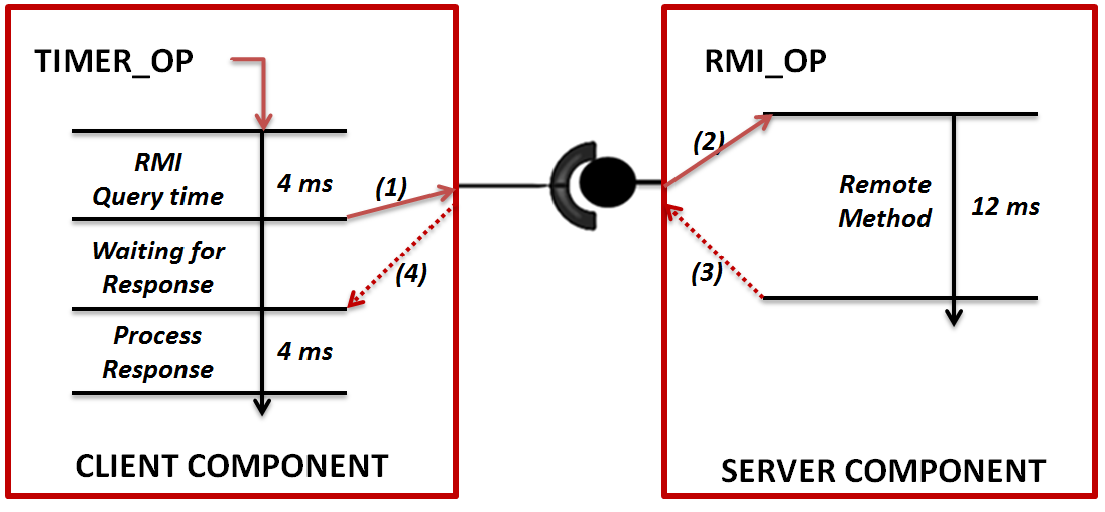
\includegraphics[width=0.4\textwidth]{rmi_application}
	\caption{RMI Application: A Periodically triggered client makes a remote method invocation to a server component. The assembly is annotated with estimated WCET on the different operational steps. The non-deterministic time here is the waiting time of the client, which is calculated using state space analysis.}
	\label{fig:rmi_application}
\end{figure}

WCET of component operational steps needs to be measured by having the component operation execute at real-time priority with no other component threads intervening this process. This measurement gives us a \emph{pure execution time} of the code block. The process must be repeated for all component operations to obtain meaningful worst-case estimates that are tailored to the target platform. Obtaining the WCET values by this method is not only more realistic but also an accurate representation of the target system. Once these individual numbers are obtained, the values are plugged into the CPN through our business-logic models. 

\begin{figure*}[h]
	\centering
	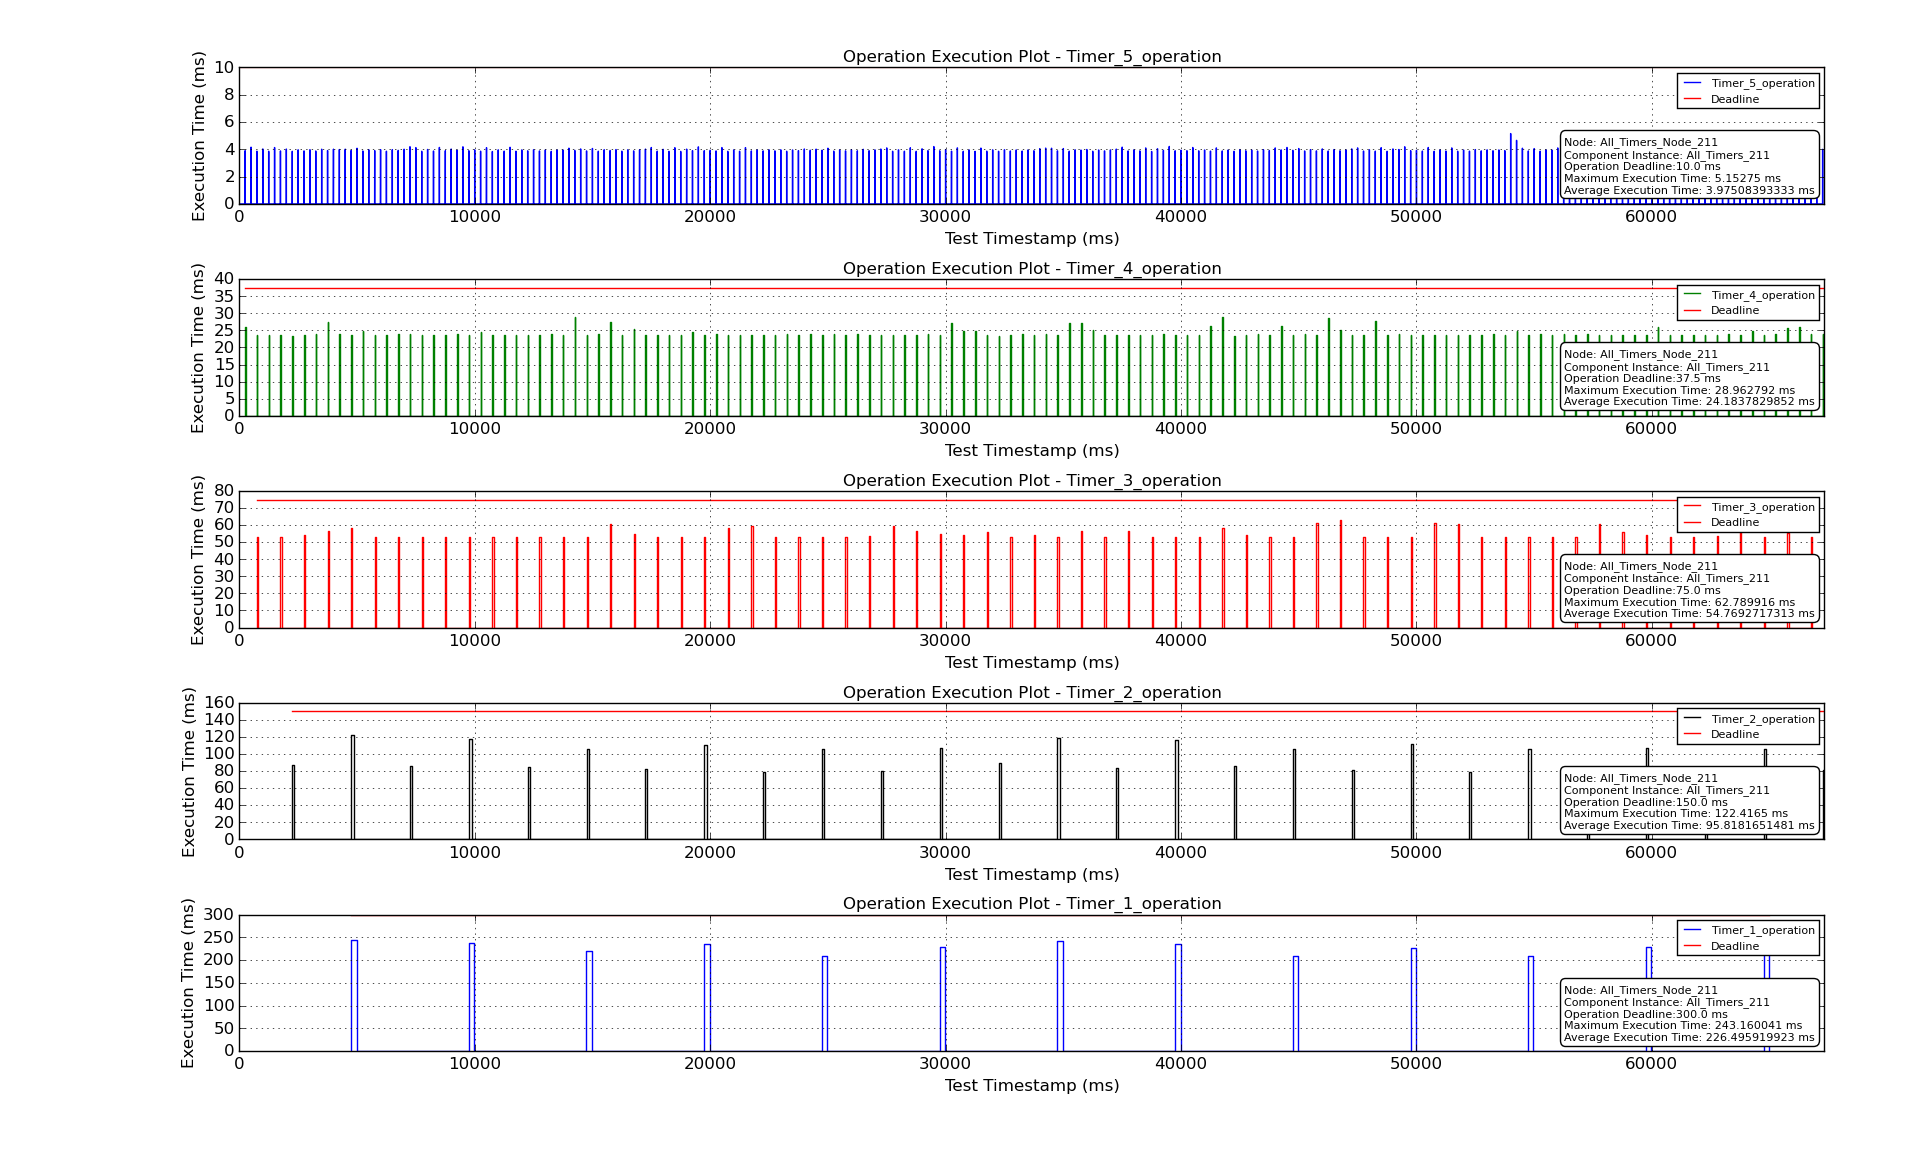
\includegraphics[width=\textwidth]{periodic-timers}
	\caption{Experimental Observation: Periodic Timers -- Five periodic timers with different frequencies and different priorities executed by a single component.}
	\label{fig:periodic-timers}
\end{figure*}

\begin{figure*}[h]
	\centering
	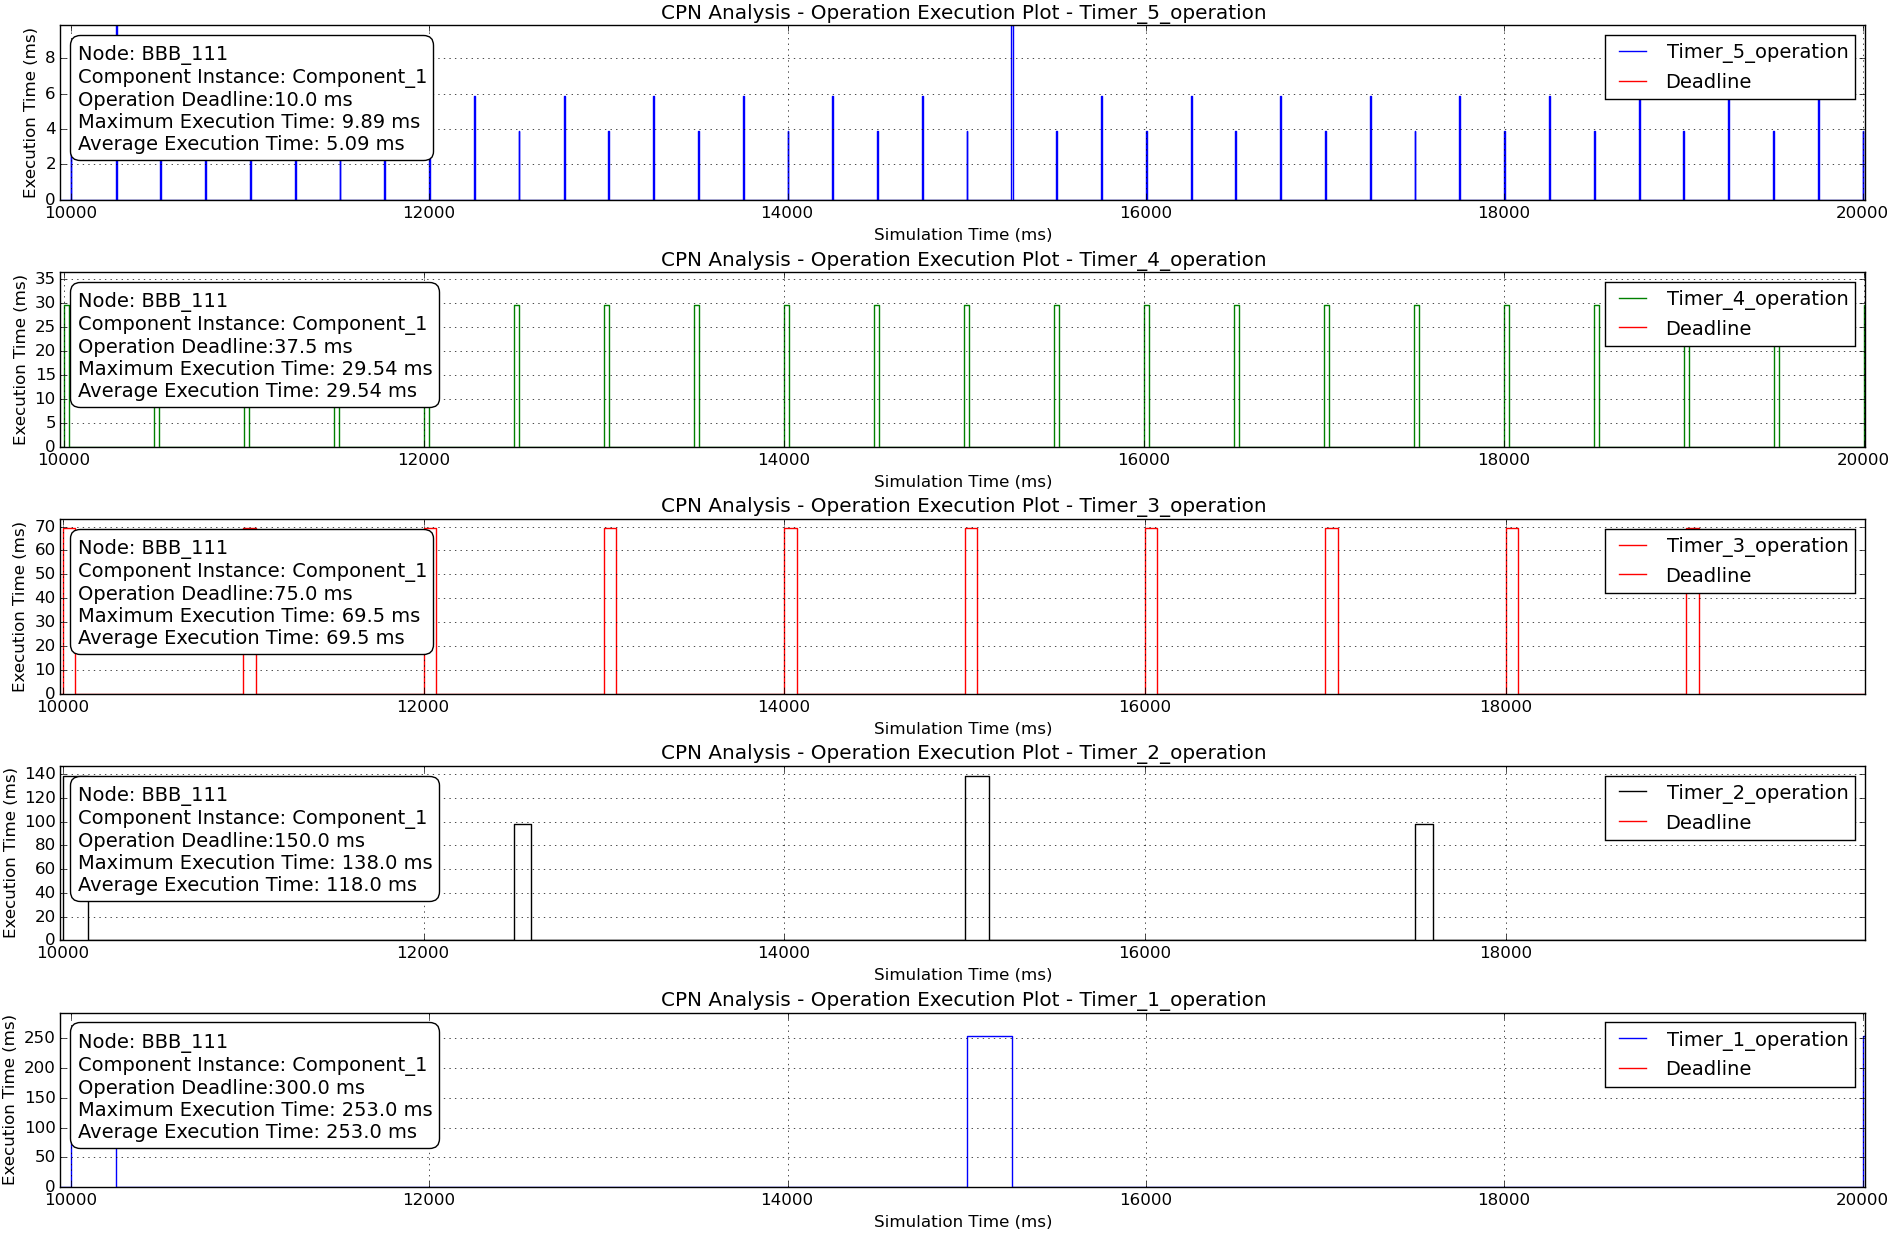
\includegraphics[width=\textwidth]{periodic-timers-cpn}
	\caption{CPN Analysis Results: Periodic Timers -- CPN state space analysis and estimation of WCET for five periodically triggered times contained by a single component. Execution time measurements for each timer is made separately and composed in the CPN model. The resultant analysis presents a conservative estimation on the WCET of the composed system.}
	\label{fig:periodic-timers-cpn}
\end{figure*}

%The remainder of this section presents some primitive interaction patterns and assemblies that have been evaluated. The presented results are restricted to some simple cases for thesake of brevity, though we have tested on medium-to-large scale examples spanning 25-30 computing nodes, and with up to a 100 components. The scalability of our model, however, is not within the scope of this paper as we have previously evaluated this metric \cite{SEUS}.

\if 0
\begin{figure*}[h]
	\centering
	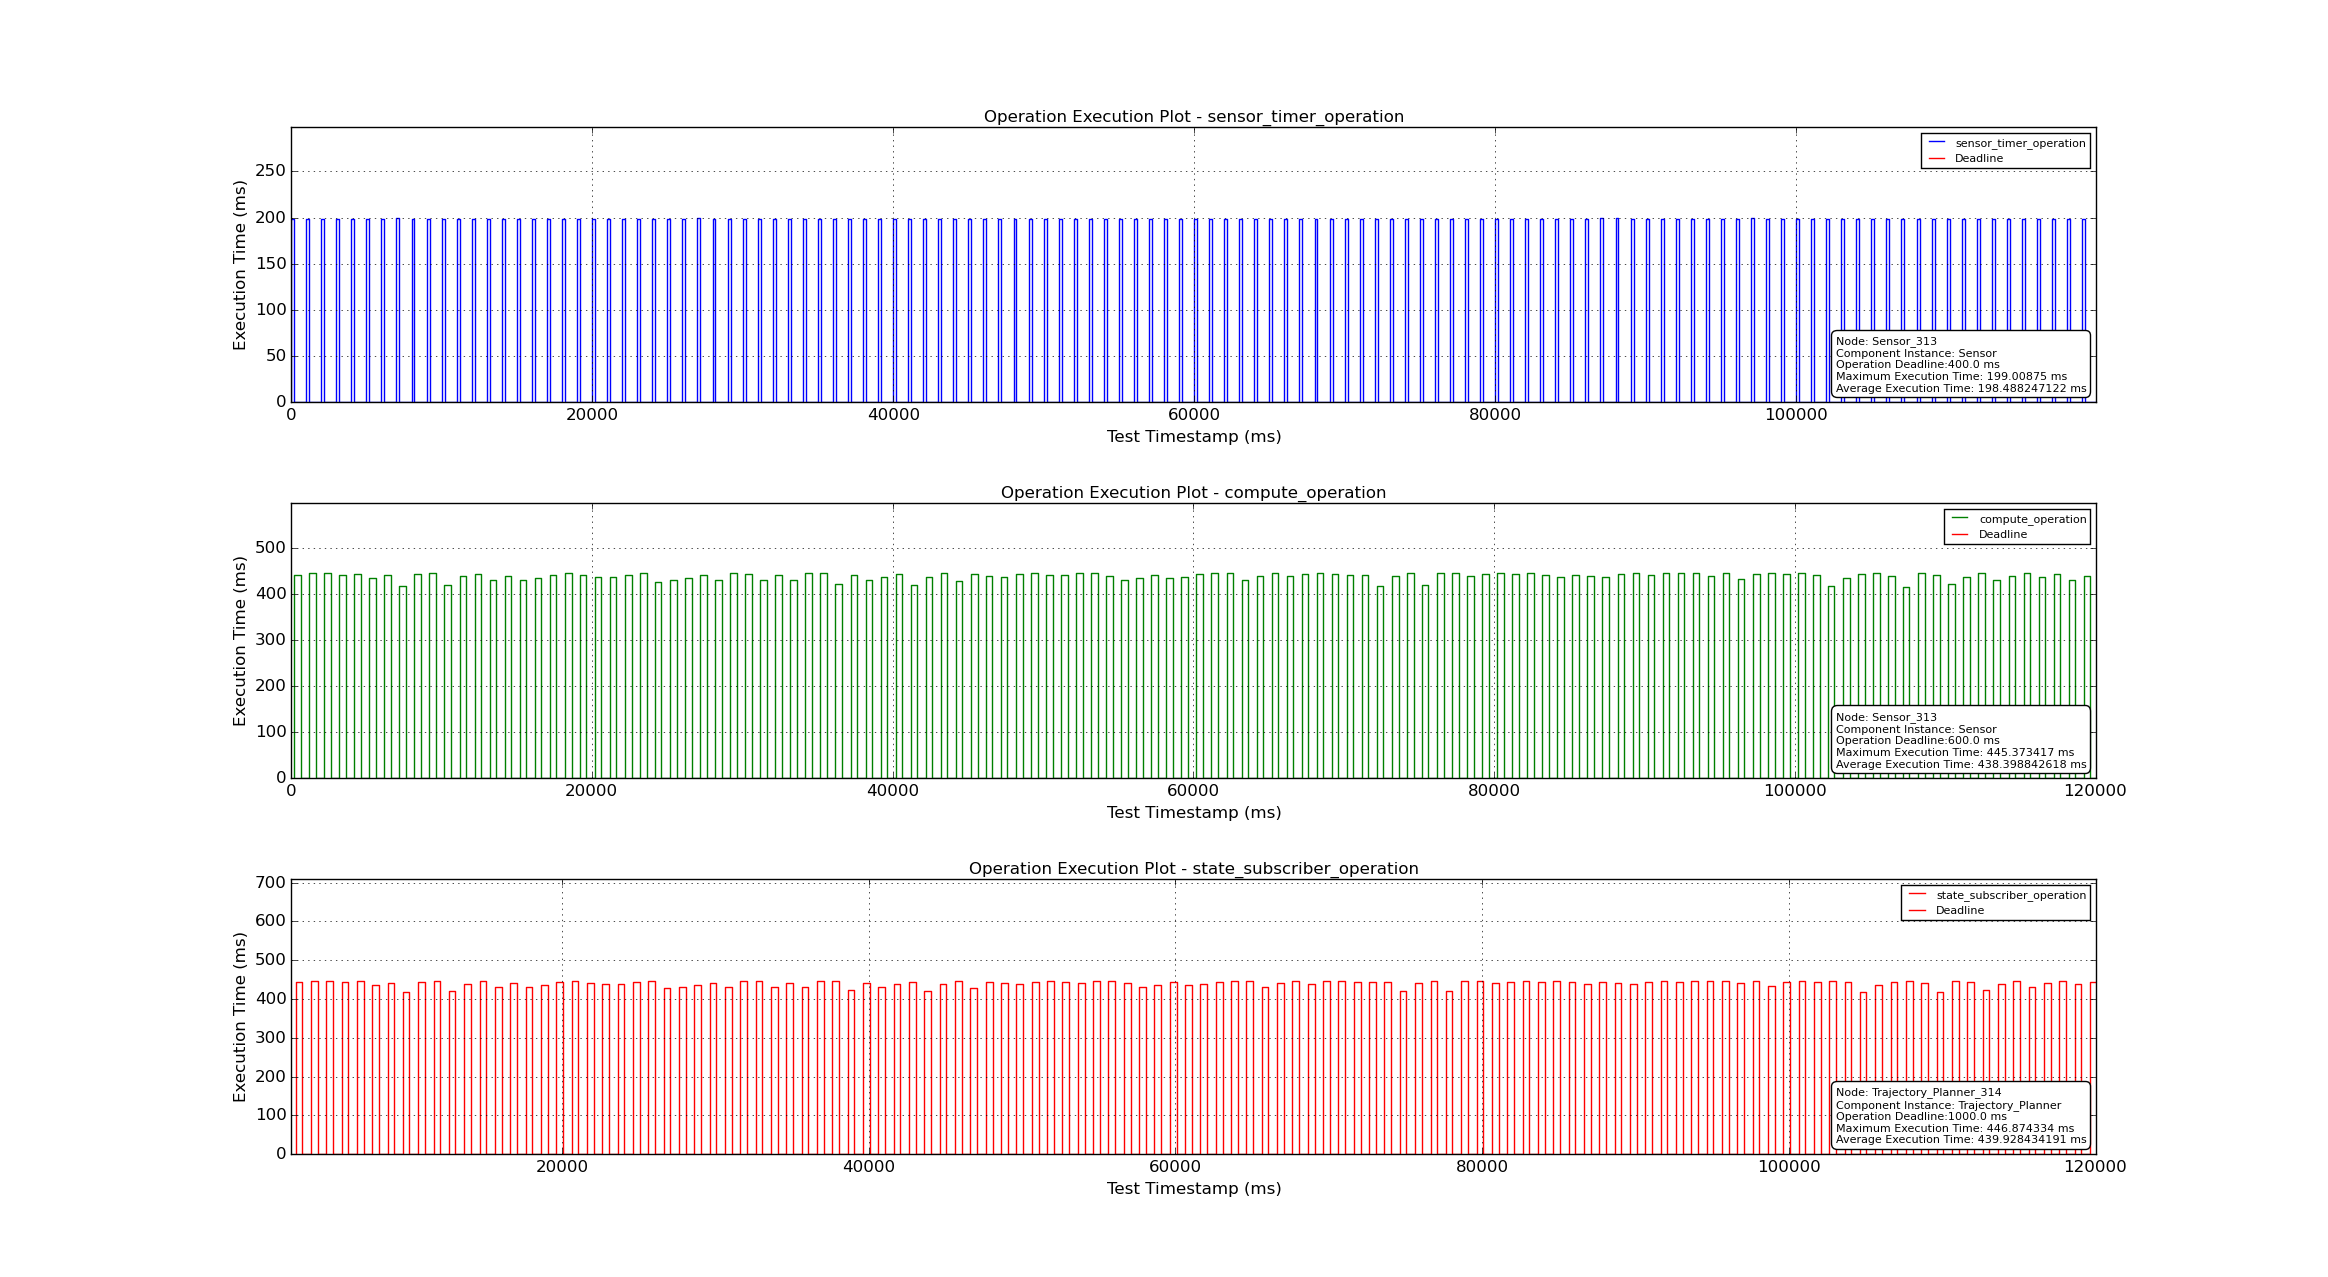
\includegraphics[width=0.75\textwidth]{trajectory-planner}
	\caption{Experimental Observation: Trajectory Planner}
	\label{fig:trajectory-planner}
\end{figure*}

\begin{figure*}
	\centering
	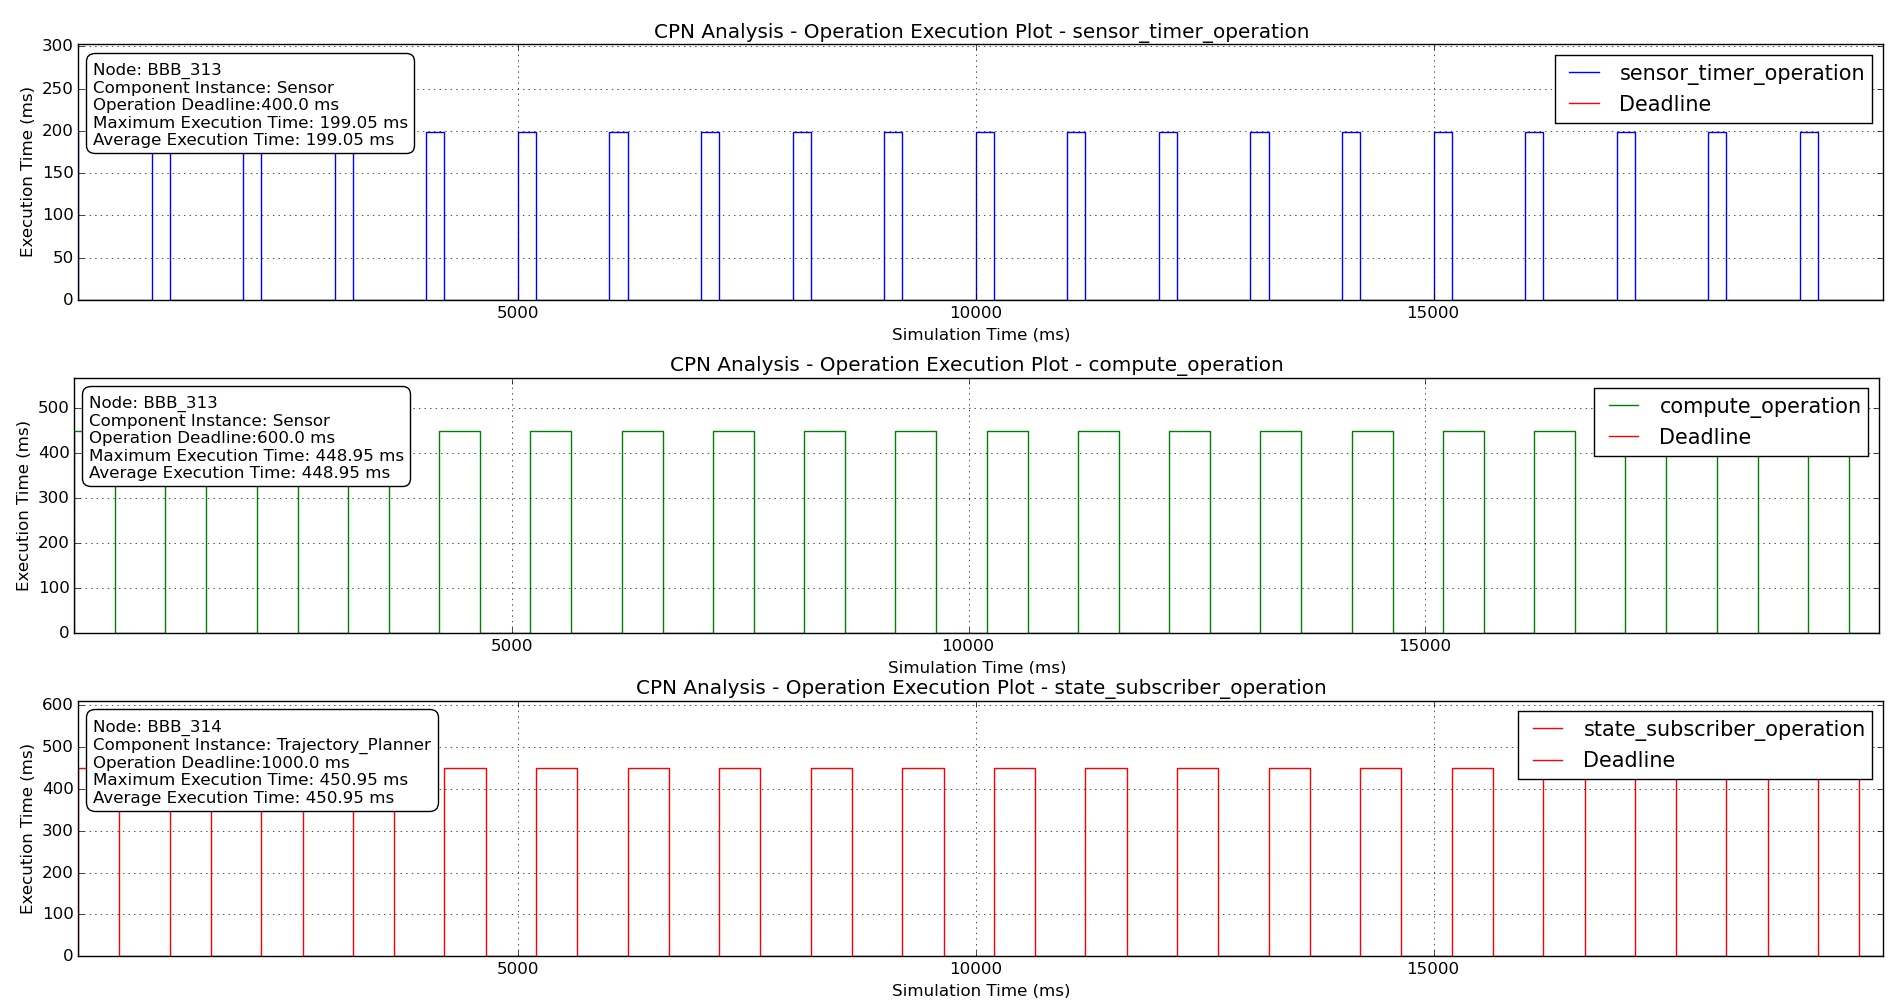
\includegraphics[width=0.75\textwidth]{trajectory-planner-cpn}
	\caption{CPN Analysis Results: Trajectory Planner}
	\label{fig:trajectory-planner-cpn}
\end{figure*}


\subsection{Trajectory Planner}

In the past \cite{kumar2014colored}, we have used a \emph{Trajectory Planner} deployment to illustrate the utility of our state space analysis. Figure \ref{fig:trajectory-planner} shows the execution time plot of this sample. A Sensor component is periodically triggered every second by the \emph{sensor\_timer} at which point it publishes a notification to the Trajectory Planner, alerting the planner of new sensor state. The planner component receives this notification on its \emph{state\_subscriber}. On receiving this message, the planner executes a remote method invocation to the \emph{compute} server located in the Sensor, blocked and waiting for a response. At this point, the \emph{compute\_operation} is executed on the Sensor which returns the updated sensor state. This unblocks the planner component which uses the new sensor state to perform trajectory planning tasks. 

This is a common interaction pattern in Cyber-Physical systems since embedded sensors are updated at a much higher frequency than a path planning entity. Thus, the planner can query the sensor at a lower rate to sample the sensor state. In this example, the planner is matching the frequency of the sensor since the execution cost is low. However, when more components are added to this deployment, the planner would have to fetch sensor state less frequently so as to not affect other system-level deadlines.  

\fi

\vspace{-0.05in}

\subsection{Time-triggered Operations}

Time-triggered operations are an integral part of our component model. ROSMOD components are dormant by default. A timer has to trigger a inactive component for all subsequent interactions to take place. Since the ROSMOD component model supports various scheduling schemes on a single component message queue, this following test evaluates a priority first-in first-out scheme. Multiple timers are created in a single component, each with a unique priority and period. A timer with a high frequency is assigned a high priority. Figure \ref{fig:periodic-timers} shows our experimental observations on a 5-timer example. 

Since ROSMOD components are associated with a single executor thread and component operations are non-preemptive, a low-priority operation could theoretically run forever, starving a higher priority operation from ever executing, leading to deadline violations e.g. \emph{Timer\_1\_operation} can affect all other higher priority timers. Figure \ref{fig:periodic-timers-cpn} shows our CPN prediction where such a scenario is evident. It can be seen that \emph{Timer\_5\_operation}, the timer with the highest priority is periodically seeing spikes in execution time, courtesy of other lower priority operations consuming CPU without preemption.

The analysis workflow, that has lead the results in Figure \ref{fig:periodic-timers-cpn}, is as follows: The time-triggered component is tested at real-time priority on the target platform, once for each timer which measures the pure execution time of each timer operation i.e. the time taken for each timer operation to execute on the target CPU without interruption. The WCET for each timer operation is then injected into our CPN analysis model and a composed timing analysis model is obtained. By performing bounded state space analysis, we derive the composed worst-case behavior of the component. Here, the execution times of each timer is affected by all other timers coupled with the execution semantics of the component model. These composed execution times will always be worse than the pure execution times due to factors like scheduling non-determinisms, context switching delays, and blocking behaviors. So, the results shown in Figure \ref{fig:periodic-timers-cpn} are the composed timing analysis results that can now be compared against the experimental observations in Figure \ref{fig:periodic-timers}. As evident in these figures, the CPN analysis results are conservative estimates of the real execution. 

%It must be noted here that the execution time values assigned to each timer operation in our CPN is the pure execution time i.e. the time taken for each timer operation to execute on the target CPU without interruption. This is the case for all operational execution times injected into the analysis model. If this is not done, then due to scheduling delays and interaction patterns, the CPN results will become gross overestimates. 

\begin{figure}[h]
	\centering
	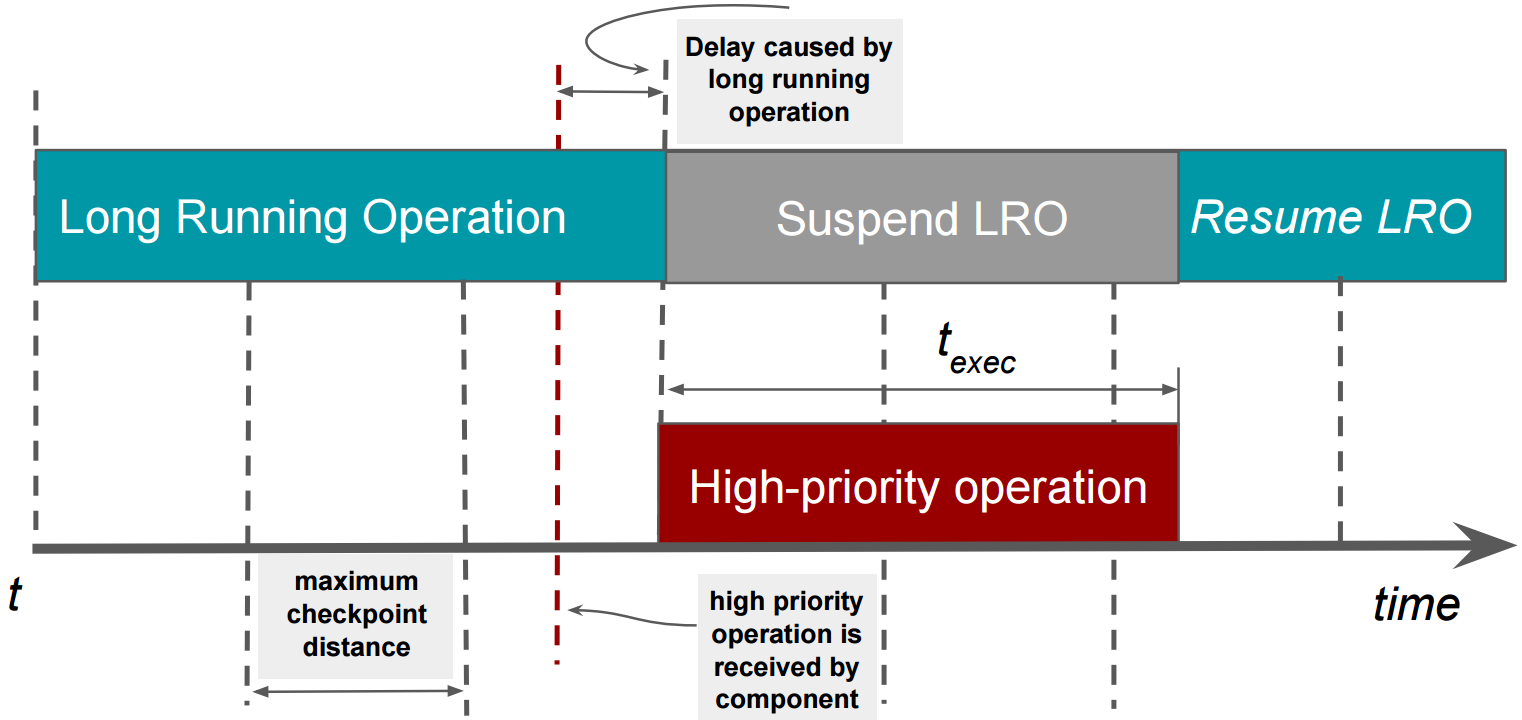
\includegraphics[width=0.5\textwidth]{lro-semantics}
	\caption{Long Running Operations (LRO) Timing Diagram -- The LRO is characterized by periodic checkpoints. At each checkpoint, the LRO checks to see if there are any higher priority operations waiting in the component message queue. If so, the LRO suspends till the higher priority operation completes and resumes and as soon as possible.}
	\label{fig:lro-semantics}
\end{figure}

\begin{figure}[h]
	\centering
	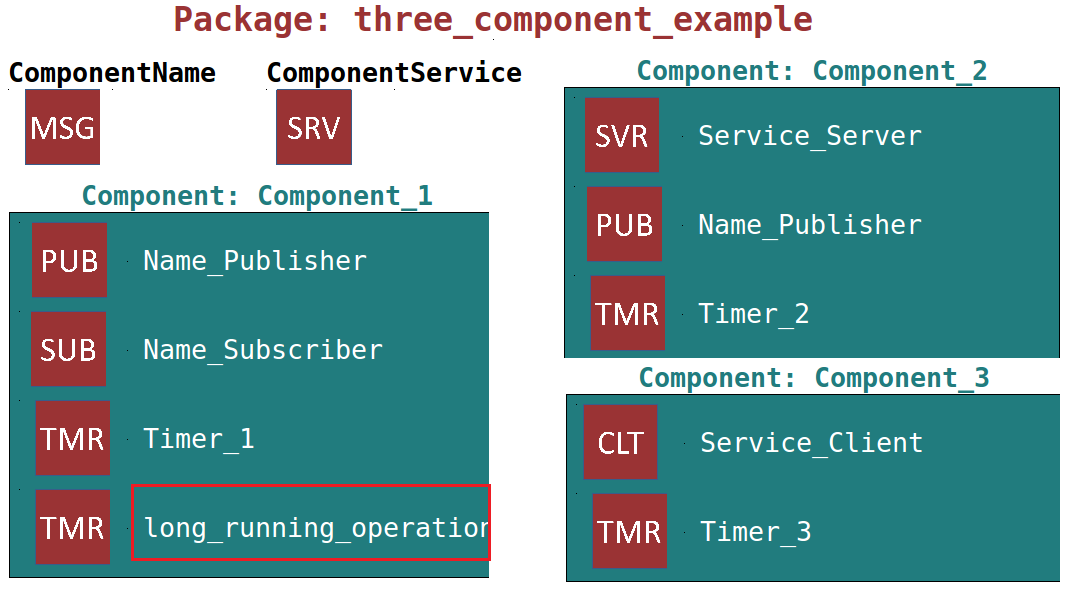
\includegraphics[width=0.4\textwidth]{three-components-lro-rosmod}
	\caption{Long Running Operation -- The Software Model consists of three components. Component\_1 contains a long running operation triggered by a sporadic timer.}
	\label{fig:three-components-lro-rosmod}
\end{figure}

\begin{figure*}[h]
	\centering
	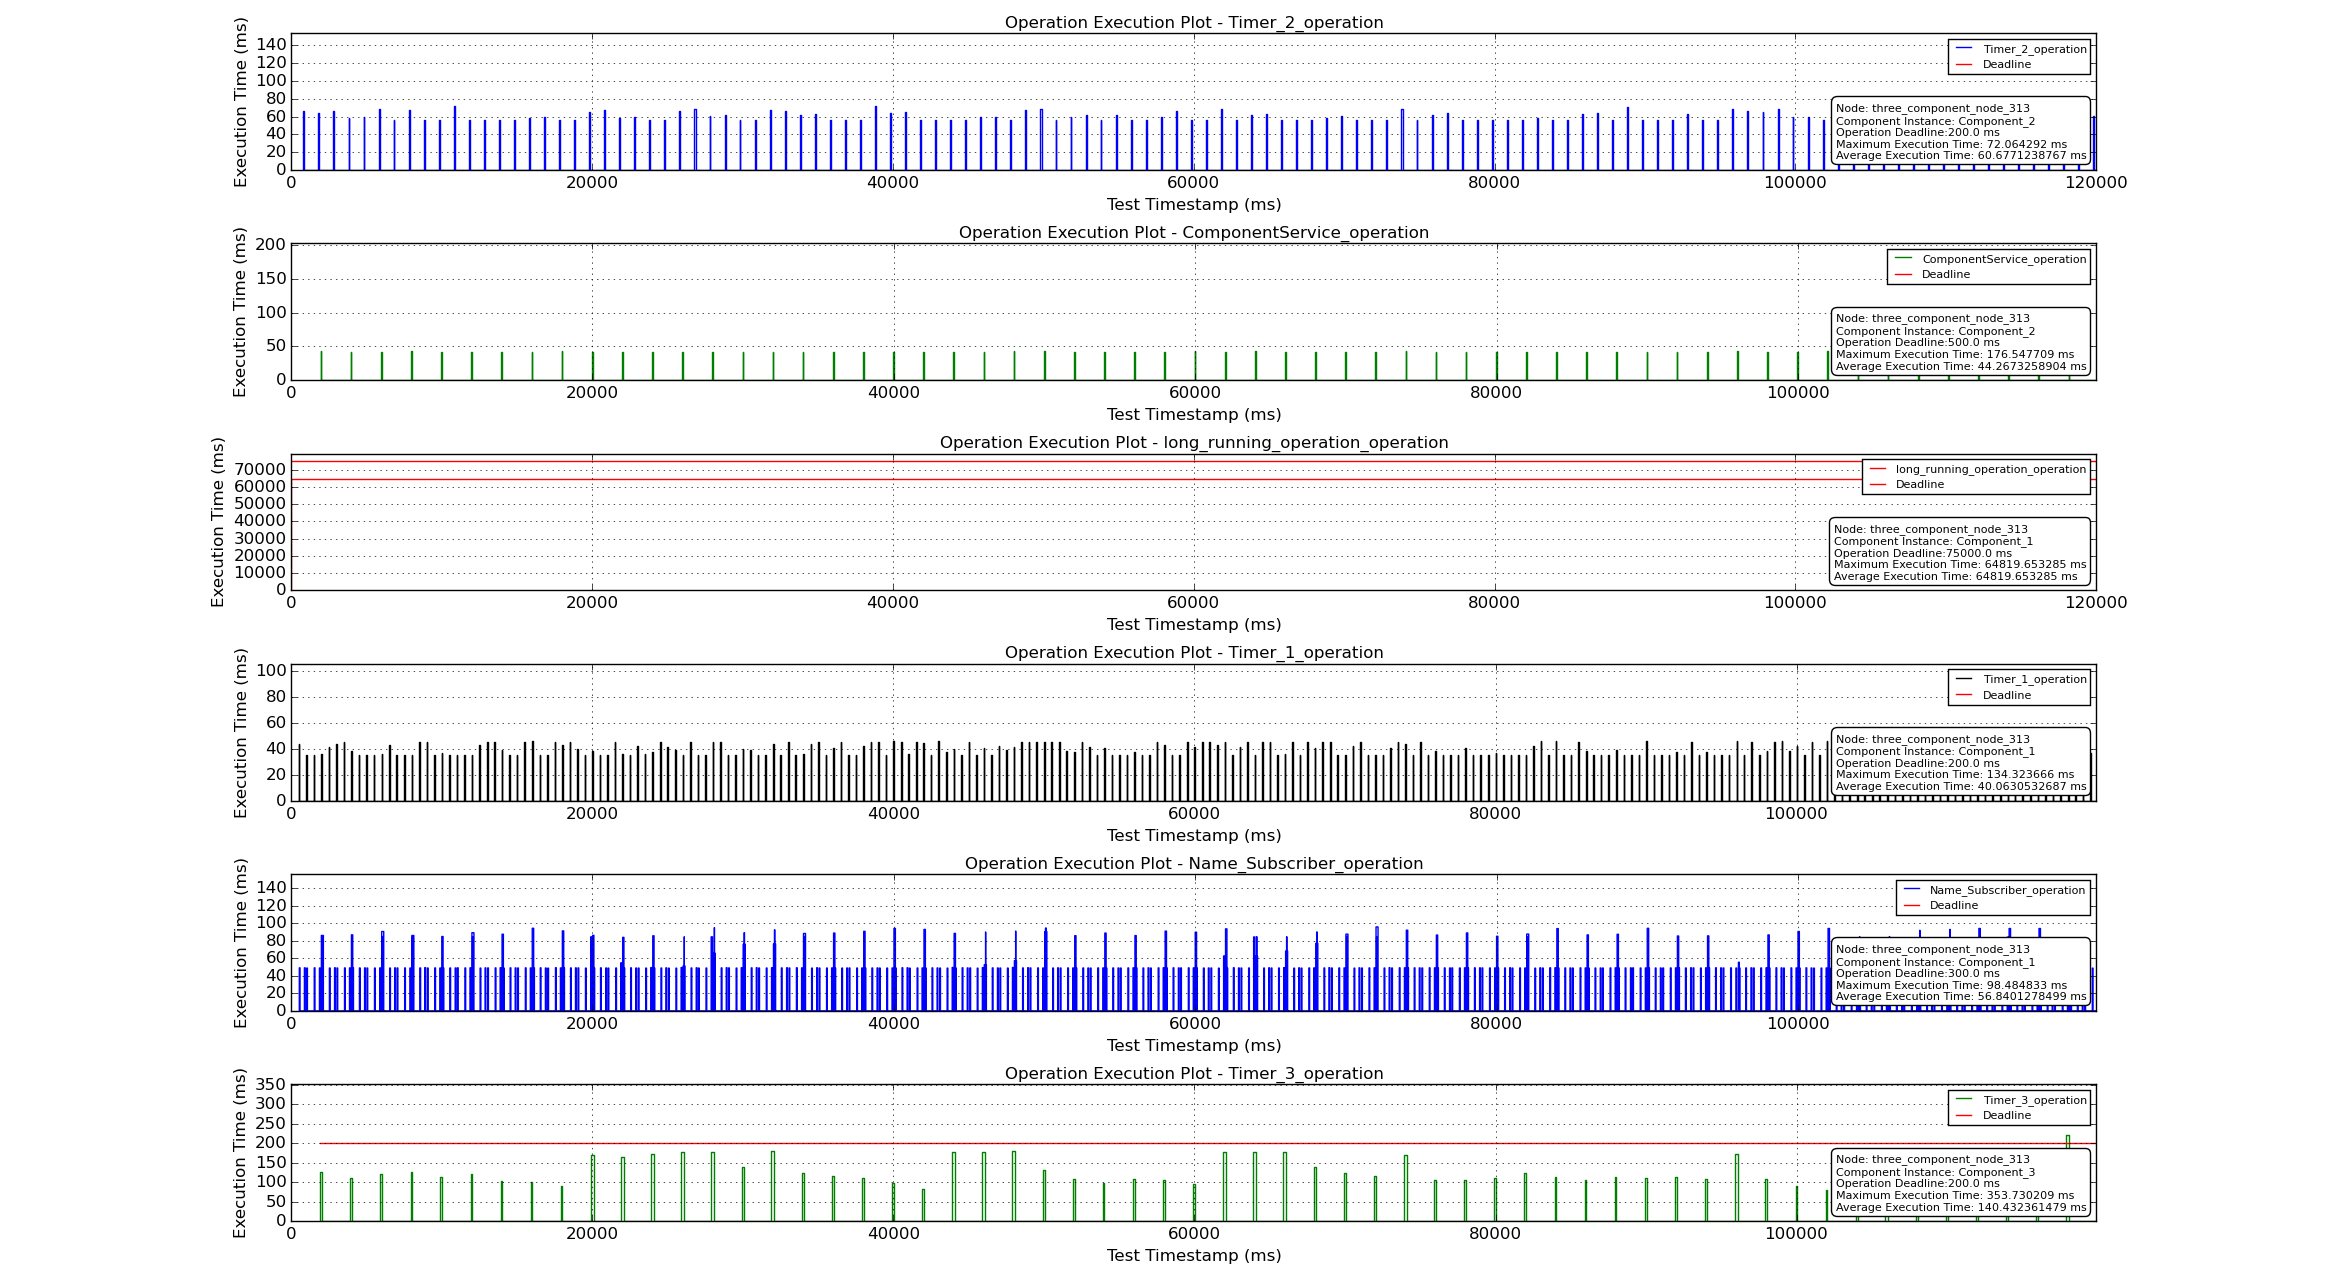
\includegraphics[width=\textwidth]{three-components-lro}
	\caption{Long Running Operations -- Experimental Observation. The goal of this test is to ensure that the long-running operation can execute concurrently in other time-triggered operations in Component\_1 and does not affect any timing properties. Periods and deadlines are chosen based on average-case performance.}
	\label{fig:three-components-lro}
\end{figure*}

\begin{figure*}[h]
	\centering
	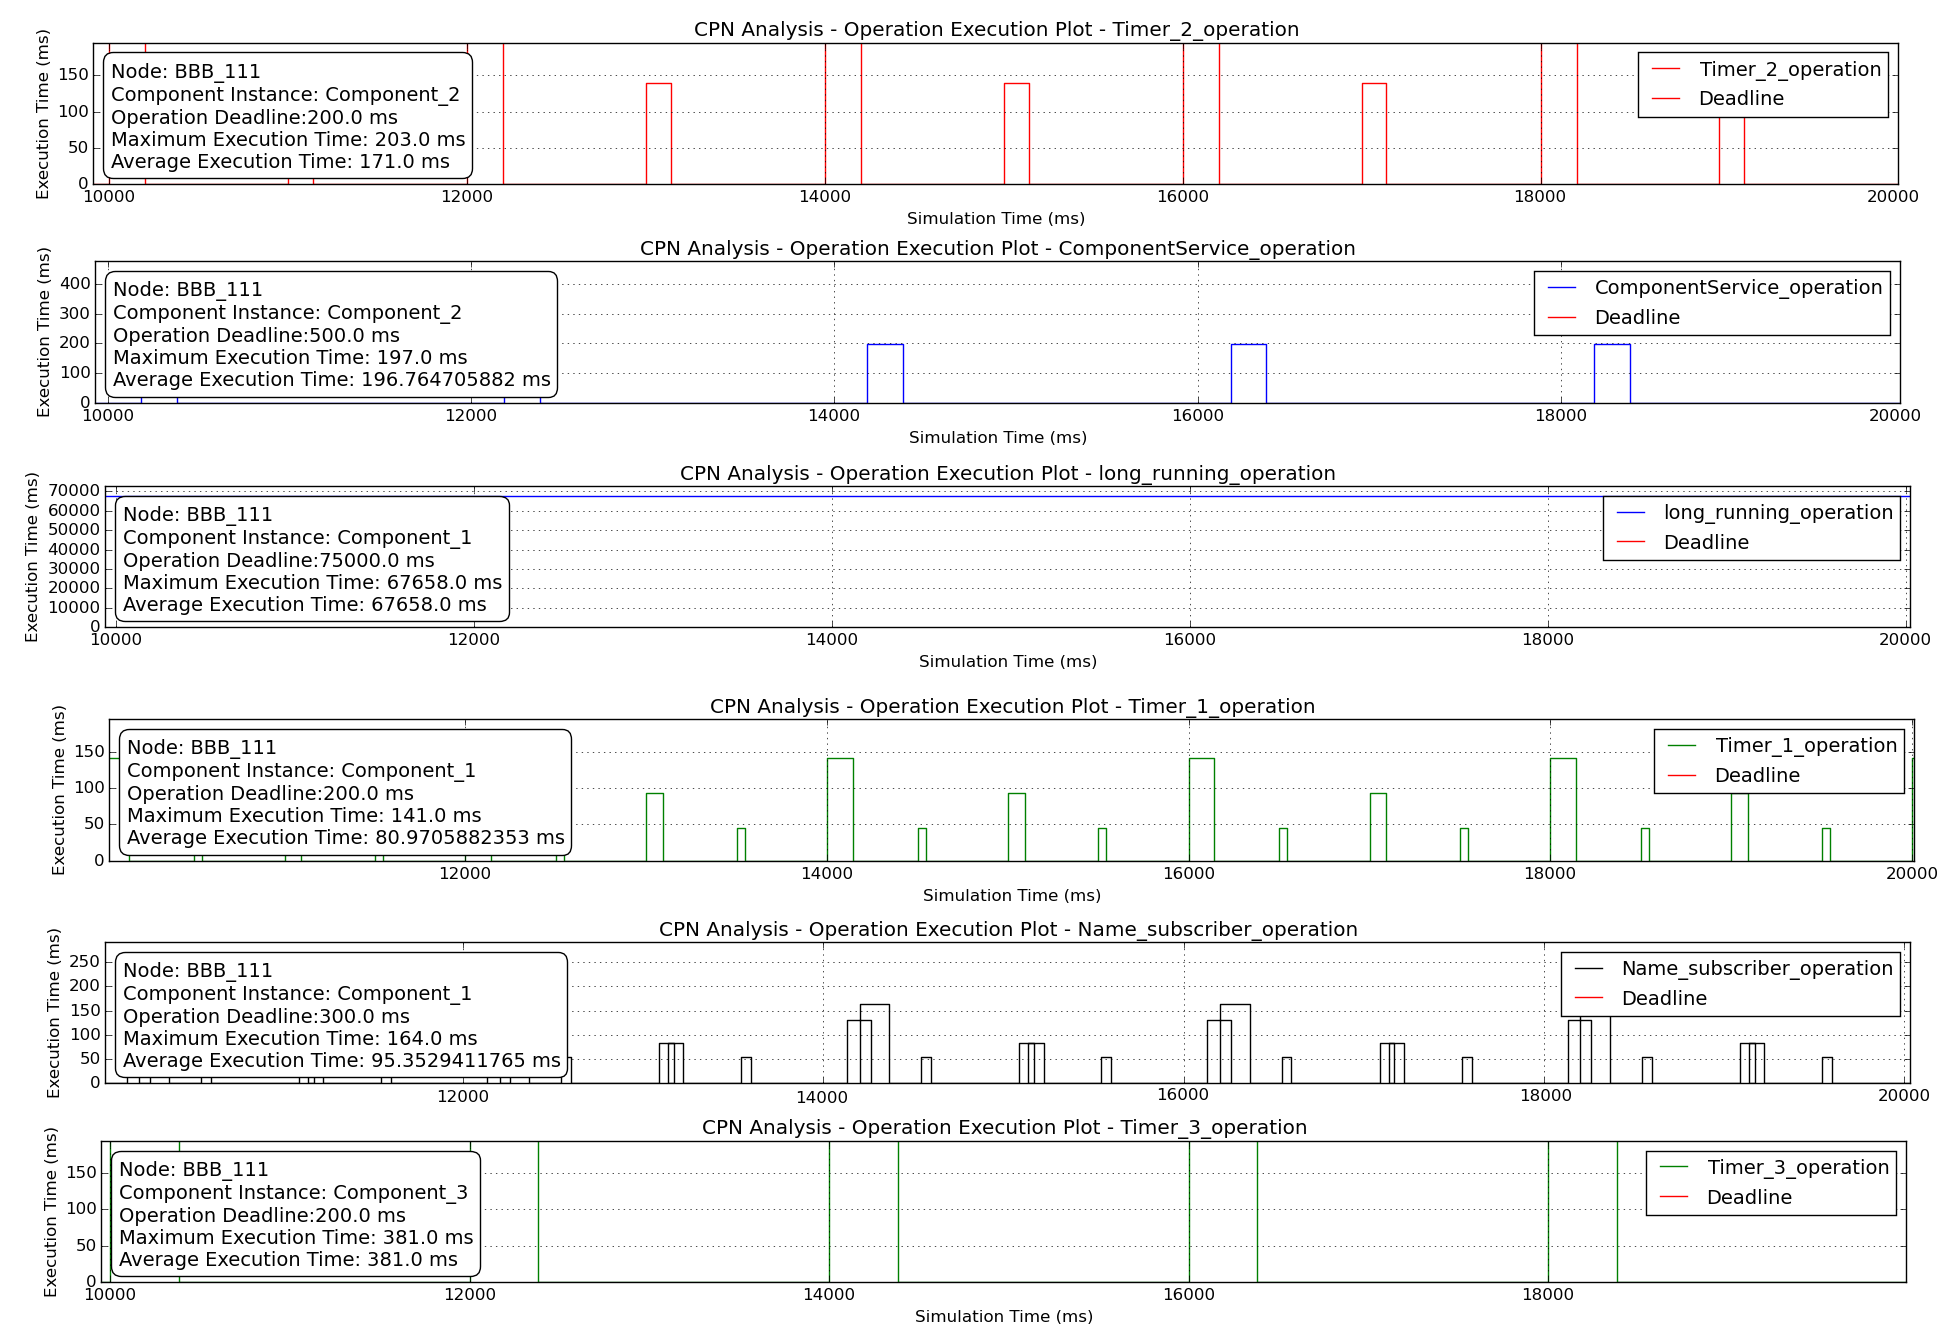
\includegraphics[width=\textwidth]{three-components-lro-cpn}
	\caption{Long Running Operations -- CPN Analysis Estimates. The CPN receives pure execution times of all operations in the component assembly from which a composed analysis is performed. The WCET plot is the representative worst-case execution trace obtained from state space analysis.}
	\label{fig:three-components-lro-cpn}
\end{figure*}

\subsection{Long-Running Operations}

Our ROSMOD component model implements a non-preemptive component operation scheduling scheme. A component operation that is in the queue, regardless of its priority, must wait for the currently executing operation to run to completion. This is a strict rule for operation scheduling and does not work best in all system designs e.g. in a long-running computation-intensive application, rejuvenating the executing operation periodically and restarting it at a previous checkpoint increases the likelihood of successfully completing the application execution. In applications executing long-running artificial intelligence (AI) search algorithms e.g. flight path planning algorithms, the computation should not hinder the prompt response requirements of highly critical operation requests such as sudden maneuver changes. Our ROSMOD component model does not support the \emph{cancellation} of long-running operations to service other highly critical operations waiting in the queue. With a few minor modifications to our scheduling schemes, long running operations can, however, be suspended if a higher priority waiting operation requires service. With these additions, we are able to model and analyze component-based systems that support long-running operations, with checkpoints, enabling the novel integration of artificial intelligence-type algorithms into our design and analysis framework. 

\subsubsection{Challenges}

One of the primary challenges here is to identify the semantics of a long-running component operation i.e. the scenarios under which the component operations scheduler suspends a cooperating long-running operation in favor of some other operation waiting in the queue. If a long-running computation is modeled as a sequence of execution steps with bounded checkpoints, then the operation would execute one step at a time and suspend at such checkpoints if necessary. An important challenge here is accurately identifying the priority difference between the long-running operation and the waiting operation. If the long-running operation is one checkpoint away from completion e.g. 100-200 ms of execution time, then strictly following our suspension rules would not be the most prudent choice since this operation is almost complete. However, if the waiting operation is a critical one, then regardless of the state of the long-running operation, the executing operation must be suspended.

\subsubsection{Implementation and Results}

In each long-running operation, we, therefore, include a synchronous \emph{checkpoint step}, as shown in Figure \ref{fig:lro-semantics}. The only assumption we make about this long-running operation is the periodicity of these checkpoint steps i.e. we know how frequently a new checkpoint is reached and we assume that the search algorithm used by the long-running operation is capable of reaching a safe state (the checkpoint) before suspending itself if required. If a higher priority operation is ready and waiting in the queue, the long-running operation runs till the next checkpoint is reached, then suspends. The higher priority operation is then processed. Figure \ref{fig:three-components-lro-rosmod} shows the \emph{Software Model} for a component assembly with long running operations.

The assembly consists of three components. Components \emph{Component\_1} and \emph{Component\_2} periodically publish on the \emph{ComponentName} message. \emph{Component\_3} periodically queries the server in \emph{Component\_2}. During these interactions, \emph{Component\_1} is performing a long running operation; the duration  of this operation is several times larger than the average execution time of all other operations. Figure \ref{fig:three-components-lro} shows the execution time plot of this scenario, as measured on our testbed. Figure \ref{fig:three-components-lro-cpn} shows our CPN analysis results for the same assembly. The plots represent the execution times of the various operation in the component assembly. As described in Section \ref{sec:ROSMOD}, execution time refers to the duration of time taken for an operation to be marked as 'complete' once it is enqueued on the component message queue. This explains the intersections in the plots for \emph{Name\_Subscriber\_operation} in \emph{Component\_1} as this is a subscriber port receiving messages on a same topic from two different publishers, in \emph{Component\_1} and \emph{Component\_2}. Secondly, it can be noted that the CPN predictions for \emph{Timer\_3\_operation} show no variation between the worst-case execution time and the average-case execution time (381.0 ms). This is because Component\_3 is not collocated with any other component and executing alone. Thus, the operation is not affected by any scheduling non-determinism or context switching delays. 
 
This exposes the conservative nature of the analysis. The Colored Petri net is an abstraction of the real execution behavior and makes several simplifications in order to obtain tractable analysis. Even still, there are analysis cases where the model is unable to perform as desired. For instance, the operating system (OS) scheduler uses a fixed-priority preemptive scheme with Round-Robin conflict resolution i.e. when two equal-priority threads are ready to execute, one is chosen at random and subsequently, Round-Robin scheduling is enforced. In the analysis, when we increase the number of equal-priority component threads, the state space of the analysis will explode since there are \emph{n!} possible thread execution orderings for \emph{n} equal priority threads executing on a device. The results of such an analysis may require searching a very large state space and may also cause a gross over-estimation of the execution times due to a single bad execution trace. This is a consequence of the simplified nature of the analysis, specifically the chosen OS scheduling model and the usage of worst-case execution times instead of other probabilistic methods. However, for strict safety-critical real-time systems that advocate predictable, deterministic behaviors, our analysis is still relevant. 
 
 \vspace{-0.1in}

%This means that the real deployment of the application threads \emph{never} exceeds the predicted worst-case execution times. Such results will validate the predicted timing properties of the system and ensure that the CPN analysis is useful and reliable.  

